\documentclass[a4paper,12pt]{article}
\usepackage[utf8]{inputenc}
\usepackage[brazil]{babel}
\usepackage{url}
%\usepackage{graphicx}
%\usepackage{graphics}

% The following is needed in order to make the code compatible
% with both latex/dvips and pdflatex.
\usepackage{ifpdf}
\ifpdf
	\usepackage[pdftex]{graphicx}
	\DeclareGraphicsRule{*}{mps}{*}{}
\else
	\usepackage[dvips]{graphicx}
\fi



\title{T2 modular}
\author{Marcelo Politzer, Raphael Bertoche}

\begin{document}

\maketitle

\section{Requisitos Funcionais}

\begin{enumerate}
\item Criar um usuário com uma UserID de até 15 caracteres, composta por [a-z;0-9;.-\_@].
  (nao vai ter comando, é acessado no menu de login.)

\item Logar com usuário já existente, que significa modificar o usuário corrente (nao é possível logar com usuário inexistente)
  (nao vai ter comando, é acessado no menu de login.)

\item Excluir perfil (busca e remoção de usuário) - delme

\item Editar perfil e interesses (Amizade, Trabalho, relacionamento aberto...)
  editme

\item Procurar filtrando por: interesse, amizade, idade, ID, nome
  search/list [-f] [-u userid] [-i interest] [-a minage-maxage] [-n name (regular expression)]
    -f - mostra apenas amigos

\item Adicionar novo contato (incluir usuário nos contatos)
  addfriend userid

\item Retirar contato (excluir usuário dos contatos)
  unfriend userid

\item Enviar mensagens para mais de um destinatário dentre os usuários já adicionados.
  write [destinatario1] [destinatario2] ... até 200

\item Arquivar mais de uma mensagem na caiza de mensagens de cada usuário

\end{enumerate}

\section{Requisitos Não Funcionais}

\subsection{Arquitetura}
\includegraphics{arch.1}

\subsection{Modelo Físico}
%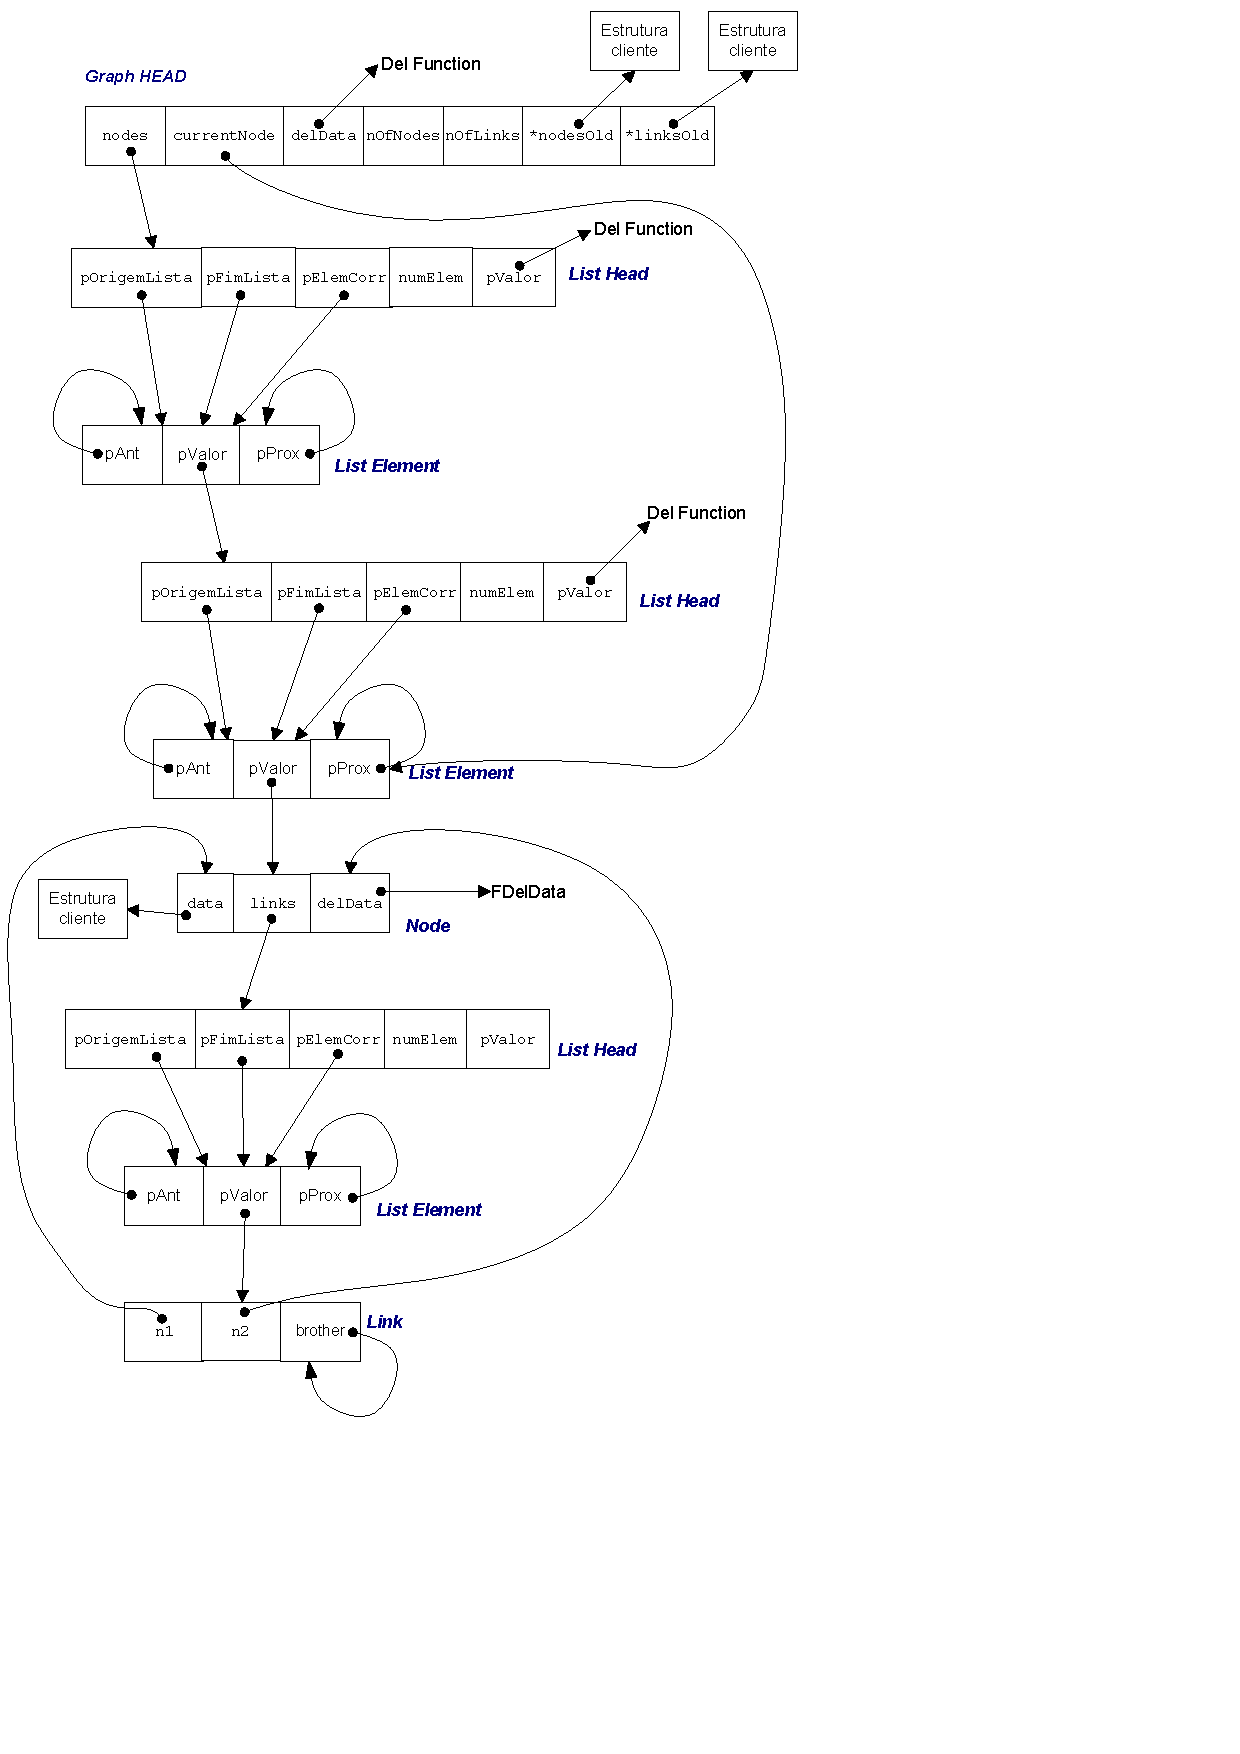
\includegraphics{fisico.1}

\subsection{Exemplo}
%\includegraphics{exemplo.1}

\end{document}
